\chapter[Klasifikácia]{Klasifikácia na základe lokálnej informácie}

\section{Úloha klasifikátora}

V našej práci sme klasifikátor použili na zakomponovaní dodatočných informácií o sekvenciách do modelu zarovnania sekvencií. Dodatočné informácie sú poskytnuté formou anotácií k príslušným bázam.

V našich modeloch sme použili 2 typy klasifikátorov -- \textit{Match klasifikátor} a \textit{InDel klasifikátor}.

Match klasifikátor sa klasifikátor určuje s akou pravdepodobnosťou sa majú dané dve pozície v sekvenciách zarovnať k sebe. Jeho výstupom je číslo z intervalu $\left<0,1\right>$, pričom čím bližšie je toto čislo k 1, tým si je klasifikátor istejší, že dané 2 pozície sa majú zarovnať k sebe. Naopak, čím bližšie je k 0, tým si je viac istý, že by tieto pozície k sebe byť nemajú.

InDel klasifikátor urcuje s akou pravdepodobnosťou má byť pozícia v príslušnej sekvencii zarovnaná s medzerou. Jeho výstupom je opäť  číslo z intervalu $\left<0,1\right>$, pričom čím bližšie je toto čislo k 1, tým si je klasifikátor istejší, že daná pozícia sa má zarovnať k medzere a čím bližšie je k 0, tým si je viac istý, že sa táto pozícia nemá zarovnať k medzere.

Tieto pravdepodobnosti sú akousi mierou istoty daného klasifikátora, a keďže tieto 2 klasifikátory sú nezávislé, súčet ich výstupov nemusí byť jedna.

\section{Vstupné dáta}

V práci sme vyskúšali a porovnali viacero typov vstupných dát a porovnali sme ako dobre sa klasifikátor na týchto dátach učí. Všetky typy dát sú založené na okne okolo daných pozícií, ktoré je definované v nasledujúcej sekcii.

Na porovnanie typov dát sme používali dve miery - významnosť \todo features a úspešnosť klasifikátora.

\subsection{Definícia okna}
\label{subsec:window}
Ako vstupné dáta dostane klasifikátor okolie okolo daných pozícií. Toto okolie budeme volať \textit{okno}. Okno veľkosti $w$ pozostáva z $2w$ blokov veľkosti $k = (1+\#\text{anotácií})$.

Majme teda dve sekvencie, $X = x_1 x_2 \dots x_n$ a $Y = y_1 y_2 \dots y_n$ a pozície $i$ a $j$.
Pri Match klasifikátore okno veľkosti $w$ obsahuje $x_{i - w/2}\dots x_i \dots x_{i + (1 + w)/2}$, $y_{j - w/2}\dots y_j \dots y_{j + (1 + w)/2}$ a všetky anotácie príslušných báz. (Obr. \ref{fig:window-m})

Pri InDel klasifikátore používame tiež dve pozície -- prvá je pozícia v inzert sekvencii a ukazuje na bázu, na ktorú sa pýtame a druhá pozícia je v druhej sekvencii a ukazuje na medzeru, teda medzi dve bázy.
Predpokladajme teraz, že $X$ je inzert sekvencia. Okno Indel klasifikátora veľkosti $w$ obsahuje $x_{i - w/2}\dots x_i \dots x_{i + (1 + w)/2}$, $y_{j - w/2}\dots y_j \dots y_{j + (1 + w)/2 - 1}$ a všetky anotácie príslušných báz. (Obr. \ref{fig:window-i})

\begin{figure}[h]
        \centering
        \begin{subfigure}[b]{0.35\textwidth}
                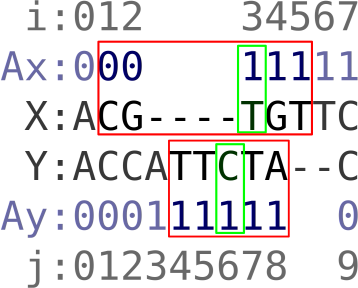
\includegraphics[width=\textwidth]{images/window_m}
                \caption{Match klasifikátor}
                \label{fig:window-m}
        \end{subfigure}%
        \qquad\qquad %add desired spacing between images, e. g. ~, \quad, \qquad etc.
          %(or a blank line to force the subfigure onto a new line)
        \begin{subfigure}[b]{0.35\textwidth}
                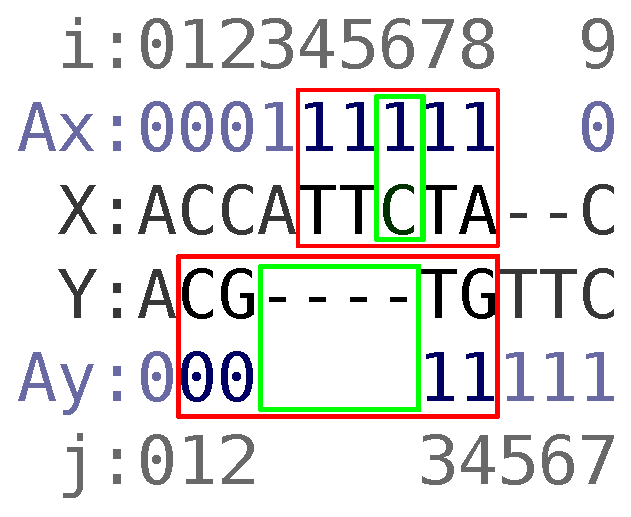
\includegraphics[width=\textwidth]{images/window_i}
                \caption{InDel klasifikátor}
                \label{fig:window-i}
        \end{subfigure}
        \caption{Okno klasifikátora pre pozície $i = 6$ a $j = 3$}
\end{figure}


\subsection{Typ dát č. 1 - okno bez úpravy}
\label{subsec:datatype1}

Ako prvý typ dát sme zobrali okno tak ako sme ho definovali v predošlej sekcii (\ref{subsec:window}). Dáta obsahujú priamo všetky bázy a anotácie tak ako sú v okne.

\todo obrazky a tabulky

% Klasifikátor sme natrénovali a zistili sme \todo ...

\subsection{Typ dát č. 2 - zhody v stĺpcoch okna}
\label{subsec:datatype2}

Druhý typ dát obsahuje aktuálnu bázu spolu s jej anotáciami a navyše pole veľkosti $k*w$, ktoré má na $i$-tom mieste 1 ak $okno_X[i] = okno_Y[i]$, ináč 0, pričom $w$ je veľkosť okna, $k$ je veľkosť bloku, $okno_X$ je časť okna zodpovedajúca $X$ sekvencii a $okno_Y$ zodpovedá $Y$-ovej časti okna.

\todo obrazky a tabulky

\subsection{Typ dát č. 3 - matica zhód v okne}

Tretí typ dát je podobný ako typ č. 2 (sekcia \ref{subsec:datatype2}), rozdiel je v tom, že teraz pole obsahuje nie len zhody po dvojiciach ale celú maticu zhôd. Teda opäť máme aktuálne bázy s anotáciami a pole má veľkosť $k*w^2$. Každý riadok sa skladá s jednotlivých blokov a v tabuľke v $x$-tom riadku, $y$-tom stĺpci a $i$-tom mieste v bloku je 1 práve
vtedy keď $okno_X[x+i] = okno_Y[y+i]$.

\todo obrazky a tabulky

\subsection{Typ dát č. 4 - kombinácia 1 a 2}

Posledný typ dát je kombináciou typov dát 1 a 2 (popísaných v sekciách \ref{subsec:datatype1} a \ref{subsec:datatype2}). Dáta opäť obsahujú všetky bázy a anotácie a navyše sme pridali pole zhód z dát typu 2. Táto informácia je síce redundantná a klasifikátor by si ju mal vedieť odvodiť aj sám, no predošlé experimenty ukázali, že by to mohlo pomôcť.

\todo obrazky a tabulky

\subsection{Zhrnutie}

\todo ktorý typ dát sa nám zdal najvhodnejší a prečo

\todo tabulky uspesnosti


\section{Trénovanie}

\subsection{Výber pozitívnych a negatívnych príkladov pre Match klasifikátor}

\subsection{Výber pozitívnych a negatívnych príkladov pre InDel klasifikátor}

% \section{Random Forest}

% \todo chcem to tu, alebo niekde inde?

% \todo



